\documentclass[a4paper]{iacas}

\usepackage{cite}
\usepackage{hyperref}% embedding hyperlinks [must be loaded after dropping]
\usepackage{amsmath,amsthm,amssymb,amsfonts,latexsym,mathrsfs,wasysym}
\usepackage{marvosym}
\usepackage{subcaption}
\usepackage{soul,color}
\usepackage{threeparttable}% tables with footnotes
\usepackage{dcolumn}% decimal-aligned tabular math columns
\usepackage{float}
\usepackage{graphicx}
\usepackage{accents}
\usepackage{tikz}
\usepackage{lastpage}
\usepackage{fancyhdr}
\usepackage{color}
\usepackage{cancel}
\usepackage{setspace}
\usepackage{enumitem}
\usepackage{pdfpages}


%\doublespacing
% or:
\onehalfspacing
%\usepackage[T1]{fontenc}
%\usepackage{bigfoot} % to allow verbatim in footnote
\usepackage[framed,numbered]{matlab-prettifier}
\pagestyle{plain}
%\usepackage[hebrew,english]{babel}
\usetikzlibrary{shapes.geometric, arrows, calc}

\newcolumntype{d}{D{.}{.}{-1}}
\graphicspath{{figures/}}

% define some commands to maintain consistency
\newcommand{\pkg}[1]{\texttt{#1}}
\newcommand{\cls}[1]{\textsf{#1}}
\newcommand{\file}[1]{\texttt{#1}}
\newcommand{\sgn}[1]{\operatorname{sgn}\left(#1\right)}
\newcommand{\sat}[1]{\operatorname{sat}\left(#1\right)}
\newcommand{\rrule}[1]{\rule[#1]{0pt}{0pt}}
\newcommand{\fracds}[2]{\frac{\displaystyle #1\rrule{-0.2em}}{\displaystyle #2\rrule{1em}}}
\newcommand{\figref}[1]{Fig.~\ref{#1}}
\newcommand{\ubar}[1]{\underaccent{\bar}{#1}}
\newcommand{\norm}[1]{\lvert \lvert \vec #1 \rvert \rvert}

%diffeomorphism

\begin{document}

\begin{center}
 \large Algorithms and Application in Computer Vision - 046746
 \end{center}
\begin{center}
\large\textbf{Homework \#2}
 \end{center}


\begin{tabular}{l}
\\
{\bf\textit{Alexander Shender 328626114}} \\
{\bf\textit{Vladimir Tchuiev 309206795}} \\
Technion - Israel Institute of Technology
\end{tabular}


\newpage
\tableofcontents
\newpage

\section{Dry section}

\subsection{Question 1.}
\subsubsection{a.}

The dimensions of the layers change in the following way:
\newline
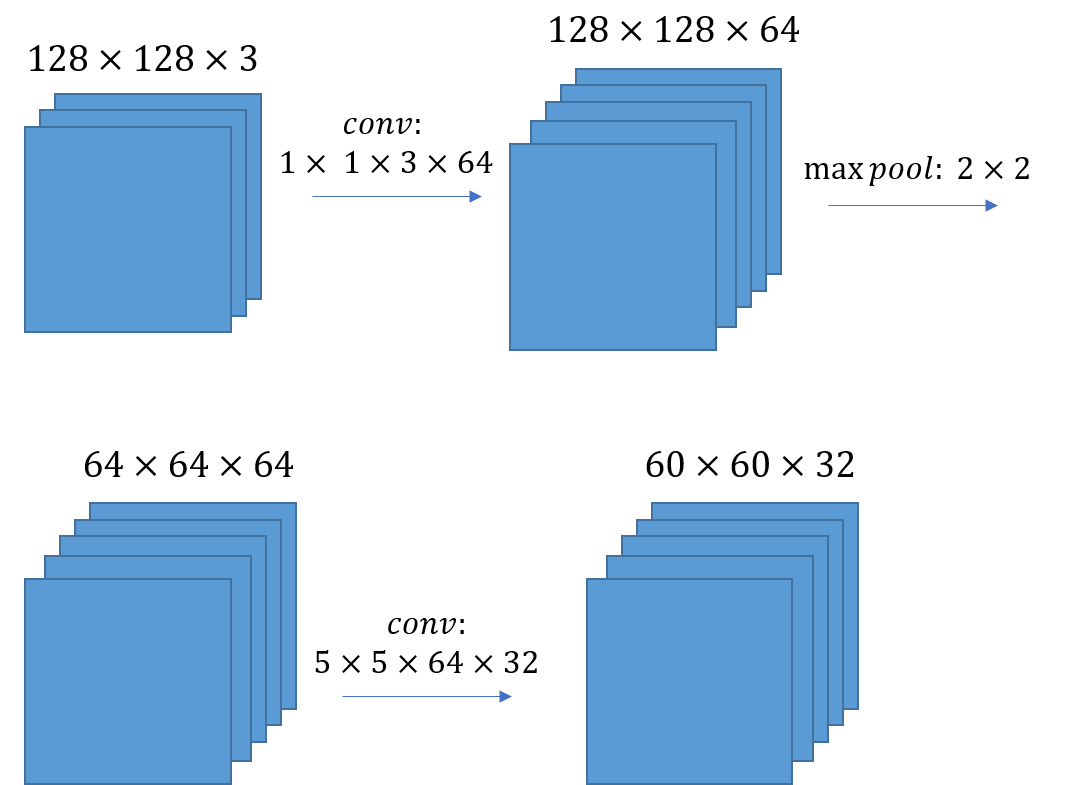
\includegraphics[scale=0.7]{imgs/q_1_1.png}
\newline
\subsubsection{b.}
The convolution of the size 1X1X(?) performs convolution on the same pixes in different channels. The input image contains 3 channels in our case, thus the convolution of the size 1X1X3 fits perfectly to result in a block of new layers without changing size (no need for padding). One kernel results in an output layer of size $128\times128$, but since we have 64 kernels, the depth of the next layers block is 64, accordingly.

\subsubsection{c.}
Let's say, our normalized filter is the following:
\begin{equation*}
\left[
\begin{matrix}
0.1 & 0.2 & 0. 05 \\
0.05 & 0.2 & 0.1 \\
0.15 & 0.1 & 0.05
\end{matrix}
\right]
\end{equation*}

We choose 2 options for stride and padding:

\begin{enumerate}
\item $stride = 2, padding = 1$
The image now has a dimensions of $9\times9$, and with a stride of 1 it gives an output dimensions: $3\times3$
\vskip 0.1in
\begin{figure}
	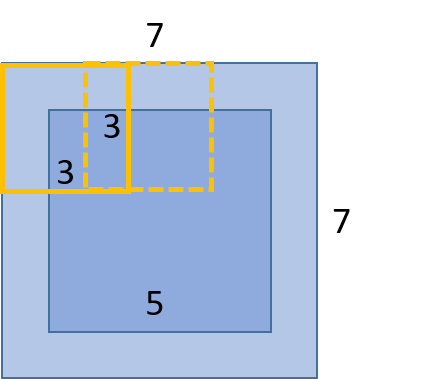
\includegraphics[scale=0.8]{imgs/q_1_31.png}
	%\caption{}
	%\label{}
\end{figure}
\vskip 0.1in

Output result is the following:

\begin{equation*}
\left[
\begin{matrix}
1.3 & 2.7 & 1.9 \\
1.9 & 5.25 & 3.1 \\
0.5 & 3.5 & 1.7
\end{matrix}
\right]
\end{equation*}


\item $stride = 1, padding = 2$
The image now has a dimensions of $7\times7$, but with stride of 2 it fits with the filter. Output dimensions: $7\times7$
\vskip 0.1in
\begin{figure}
	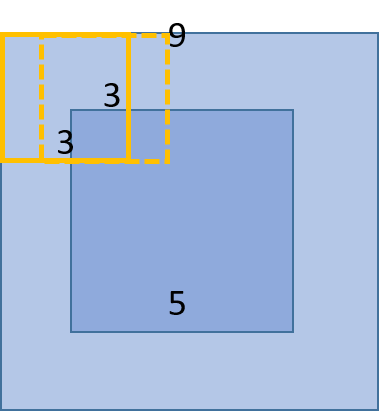
\includegraphics[scale=0.8]{imgs/q_1_32.png}
	%\caption{}
	%\label{}
\end{figure}
\vskip 0.1in

Output result is the following:

\begin{equation*}
\left[
\begin{matrix}
0.2 & 0.45 & 1 & 0.8 & 1.15 & 0.45 & 0.45 \\
0.55 & 1.3 & 2.0 & 2.7 & 2.65 & 1.9 & 0.45 \\
0.6 & 2.1 & 3.3 & 5.15 & 4.6 & 2.6 & 1.45\\
0.4 & 1.9 & 3.75 & 5.25 & 5.145 & 3.1 & 1 \\
0.2 & 1.3 & 3.5 & 4.7 & 4.0 & 3.35 & 1.45\\
0.05 & 0.5 & 2.05 & 3.5 & 2.55 & 1.7 & 0.5 \\ 
0 & 0.05 & 0.5 & 1.5 & 1.6 & 1.2 & 0.4
\end{matrix}
\right]
\end{equation*}
\end{enumerate}.
Those results were obtained using Python. The code is placed here: 'python\_code/hw2\_q1.py'.


\newpage
\subsection{Question 2.}
The architecture selected is the VGG16 architecture. The image found in the internet which describes the structure is the following:


\vskip 0.1in
\begin{figure}
	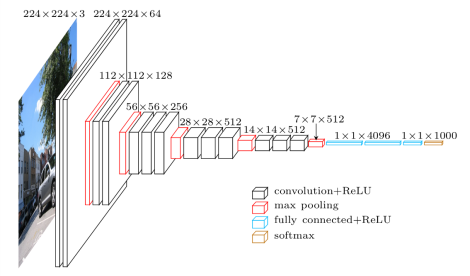
\includegraphics[scale=0.6]{imgs/vgg_arc.PNG}
	%\caption{}
	%\label{}
\end{figure}
\vskip 0.1in

Writing the exact outputs for every layer:

\begin{table}[]
\begin{tabular}{|l|l|l|l|l|l}
\cline{1-5}
Operation       & Size                   & Padding   & Stride & Output size       &  \\ \cline{1-5}
Conv block      & {[}3X3X3{]}X64         & {[}1 1{]} & 1      & {[}224X224X64{]}  &  \\ \cline{1-5}
Conv block      & {[}3X3X64{]}X64        & {[}1 1{]} & 1      & {[}224X224X64{]}  &  \\ \cline{1-5}
Pool 2D         & {[}2 2{]}              & N/A       & N/A    & {[}112X112X64{]}  &  \\ \cline{1-5}
Conv block      & {[}3X3X64{]}X128       & {[}1 1{]} & 1      & {[}112X112X128{]} &  \\ \cline{1-5}
Conv block      & {[}3X3X128{]}X128      & {[}1 1{]} & 1      & {[}112X112X128{]} &  \\ \cline{1-5}
Pool 2D         & {[}2 2{]}              & N/A       & N/A    & 56X56X128         &  \\ \cline{1-5}
Conv block      & {[}3X3X128{]}X256      & {[}1 1{]} & 1      & {[}56X56X256{]}   &  \\ \cline{1-5}
Conv block      & {[}3X3X256{]}X256      & {[}1 1{]} & 1      & {[}56X56X256{]}   &  \\ \cline{1-5}
Conv block      & {[}3X3X256{]}X256      & {[}1 1{]} & 1      & {[}56X56X256{]}   &  \\ \cline{1-5}
Pool 2D         & {[}2 2{]}              & N/A       & N/A    & {[}28X28X256{]}   &  \\ \cline{1-5}
Conv block      & {[}3X3X256{]}X512      & {[}2 2{]} & 1      & {[}28X28X512{]}   &  \\ \cline{1-5}
Conv block      & {[}3X3X512{]}X512      & {[}2 2{]} & 1      & {[}28X28X512{]}   &  \\ \cline{1-5}
Conv block      & {[}3X3X512{]}X512      & {[}2 2{]} & 1      & {[}28X28X512{]}   &  \\ \cline{1-5}
Pool 2D         & {[}2 2{]}              & N/A       & N/A    & {[}14X14X512{]}   &  \\ \cline{1-5}
Conv block      & {[}3X3X512{]}X512      & {[}1 1{]} & 1      & {[}14X14X512{]}   &  \\ \cline{1-5}
Conv block      & {[}3X3X512{]}X512      & {[}1 1{]} & 1      & {[}14X14X512{]}   &  \\ \cline{1-5}
Conv block      & {[}3X3X512{]}X512      & {[}1 1{]} & 1      & {[}14X14X512{]}   &  \\ \cline{1-5}
Conv block      & {[}3X3X512{]}X512      & {[}1 1{]} & 1      & {[}14X14X512{]}   &  \\ \cline{1-5}
Pool 2D         & {[}2 2{]}              & N/A       & N/A    & {[}7X7X512{]}     &  \\ \cline{1-5}
Fully connected & {[}7$\cdot$7$\cdot$512{]}X4096 & N/A       & N/A    & {[}1X1X4096{]}    &  \\ \cline{1-5}
Fully connected & {[}4096X4096{]}        & N/A       & N/A    & {[}1X1X4096{]}    &  \\ \cline{1-5}
Fully connected & {[}4096X1000{]}        & N/A       & N/A    & {[}1X1X1000{]}    &  \\ \cline{1-5}
\end{tabular}
\end{table}

\newpage
\subsection{Question 3.}
\textbf{Definition: }Overfitting - is a situation, where network is fitted too much to the training data, and finds it difficult to generalize to create predictions for the new data. 
\newline
\textbf{How to spot: }First of all, a researcher will notice that the accuracy of the model on the Test Dataset decreases, while the accuracy on the Training Set will still be increasing. The typical graph vizuasing error on the Test \& Training set may be seen, demonstrating this exact situation:
\newline


\vskip 0.1in
\begin{figure}
	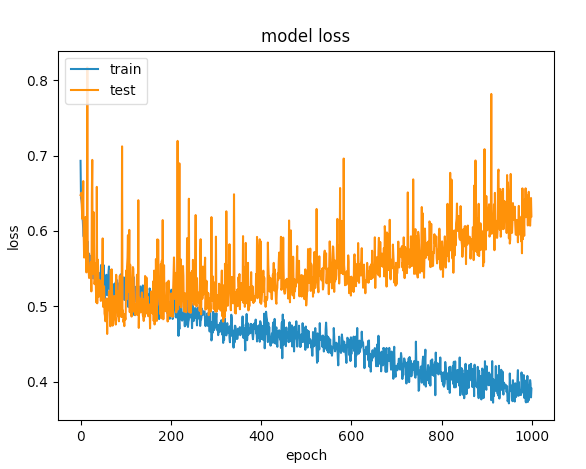
\includegraphics[scale=0.4]{imgs/overfit.PNG}
	%\caption{}
	%\label{}
\end{figure}
\vskip 0.1in


\textbf{How to avoid: }There are numerous way to avoid overfitting:
\begin{enumerate}
\item Stop the training before the accuracy for the validation set starts increasing. If the accuracy does not satisfy, find a better dataset / improve the network / apply other changes. Training for more time will worsen the situation.
\item Use one of the following methods: regularisation, lambda factor, dropout, etc.
\item Increase the dataset size. Feed the network new examples for learning.
\end{enumerate}







\newpage
\subsection{Question 4.}
The learned parameters are being updated using the backpropagation algorithm. The name derives from the way that the Error value propagates backward through the network, affecting the parameters according to the contribution that those gave to the error value. In the general view, this may be seen in update function for the parameters (in this case - weights):

\begin{equation*}
W := W - \alpha\cdot\frac{\delta E}{\delta W}
\end{equation*}
where:
\begin{align*} 
W &- \text{lweight parameter} \\
\alpha &- \text{learning rate} \\
\frac{\delta E}{\delta W} &- \text{"contribution" of the parameter to the loss}
\end{align*}

\newpage
\subsection{Question 5.}
\paragraph{\textbf{Definition:}}Batch normalization - is a method which is used to normalize the layer inputs, in order to solve the problem called \textit{internal covariate shift}. 

\paragraph{\textit{internal covariate shift:}}
the problem which arises in the intermediate layers during training because the distribution of the activations is constantly changing during training. This slows down the training by requiring lower learning rates and careful parameter initialization, and makes it notoriously hard to train models with saturating nonlinearities. \footnote{Batch Normalization: Accelerating Deep Network Training by Reducing Internal Covariate Shift , Sergey Ioffe, Christian Szegedy} \footnote{Towards Data Science: Batch normalization: theory and how to use it with Tensorflow}
\newline

So, actually we force the input of a specific layer to have approximately the same distribution in every training step. The batch normalization is performed in 4 steps (image taken from the original article):



\vskip 0.1in
\begin{figure}
	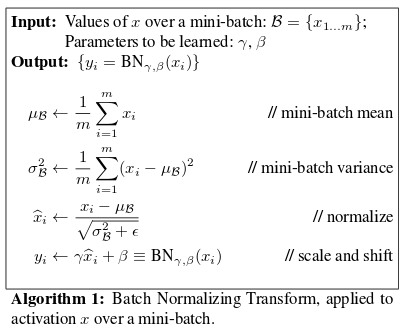
\includegraphics[scale=0.6]{imgs/batch_norm.PNG}
	%\caption{}
	%\label{}
\end{figure}
\vskip 0.1in

Steps are the following:
\begin{enumerate}
\item Calculate the batch mean of the values $x$ of a particular layer (that we do the normalization on) $\mu_{\beta}$
\item Similarly, calculate the variance of those values $x$ for this layer $\sigma_{\beta}^{2}$
\item Normalize the values, substracting the mean $\mu_{\beta}$ and dividing by STD (+constant) $\sqrt{\sigma_{\beta}^{2} + \epsilon}$. This will result in a new Gaussian distribution with mean of 0 and Variance of 1. 
\item Scale and Shift by learnable parameters $\gamma$ and $\beta$. Those parameters are being learned, and are inserted to make it possible to the distribution to be scaled and shifted if such is needed. For example, if it is of our interest to make the batch normalization an identity transform. 
\end{enumerate}

\newpage



\section{Wet section}

\subsection{Question 1.}
The subsection numbers here do not match the numbers as in the questions booklet, but the order is correct. In order to run the code for this question, run the .py file :  'python\_code/mnist\_pytorch.py'.  The script will automatically create the data folder (where the MNIST dataset will be downloaded), and the results folder (according to the current time in :day:hour:minute: format), where all the graphs which are presented here will be placed.

\subsubsection{\textbf{a.}}
\textbf{This subsection answers the steps 1-6. }
\newline
Network is the following:
\begin{itemize}
\item Network as defined in step 2
\item Loss function = CE (Cross Entropy)
\item Optimizer: SDGM (momentum = 0.5)
\item Learning rate = 0.01
\item Epochs = 8
\item Training minibatch size = 128
\item Training/validation split = 50000/10000.  (MNIST dataset includes 60000 examples)
\end{itemize}

Answering the step 5 question:

\begin{enumerate}
\item Loss value graphs:

\vskip 0.1in
\begin{minipage}{\linewidth}
	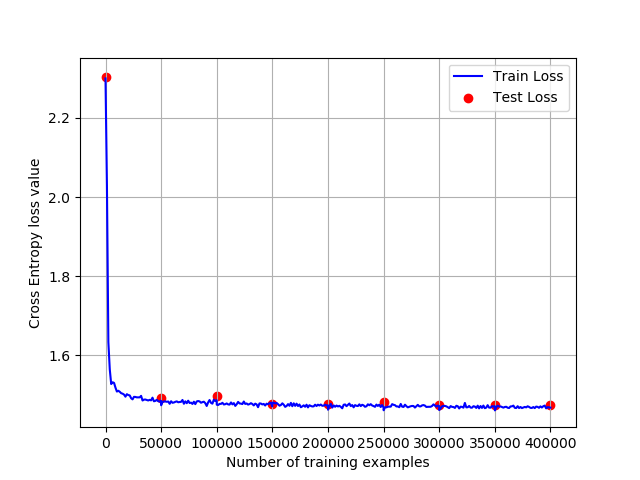
\includegraphics[scale=0.8]{hw2_py/results/_14_01_43/lr_0_01_net_1_CE_/loss_value.png}
	\captionof{figure}{Loss value as a function of the training examples seen}
	\label{fig_1}
\end{minipage}
\vskip 0.1in
\begin{minipage}{\linewidth}
	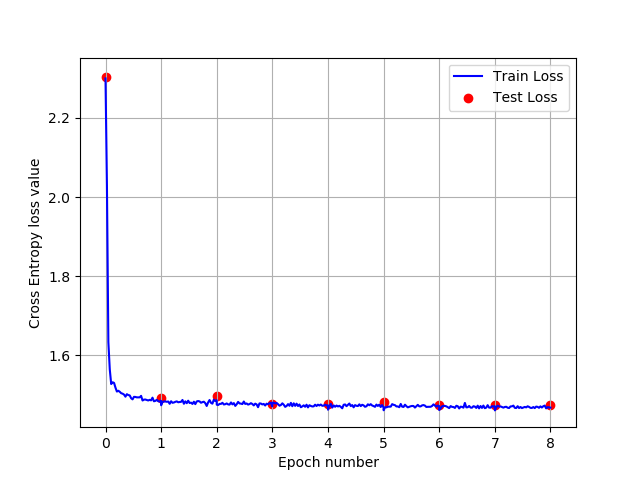
\includegraphics[scale=0.8]{hw2_py/results/_14_01_43/lr_0_01_net_1_CE_/loss_value_epoch.png}
	\captionof{figure}{Loss value as a function of the Epoch number}
	\label{fig_2}
\end{minipage}
\vskip 0.1in


\item Classification accuracy graphs

\vskip 0.1in
\begin{minipage}{\linewidth}
	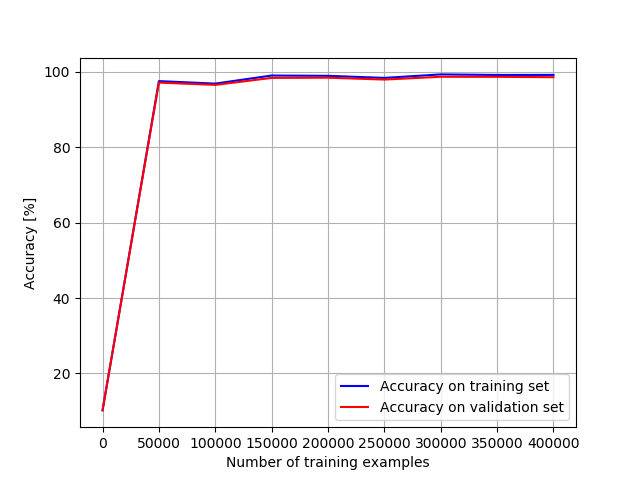
\includegraphics[scale=0.8]{hw2_py/results/_14_01_43/lr_0_01_net_1_CE_/accuracy.png}
	\captionof{figure}{Classification accuracy as a function of the training examples seen}
	\label{fig_3}
\end{minipage}
\vskip 0.1in
\begin{minipage}{\linewidth}
	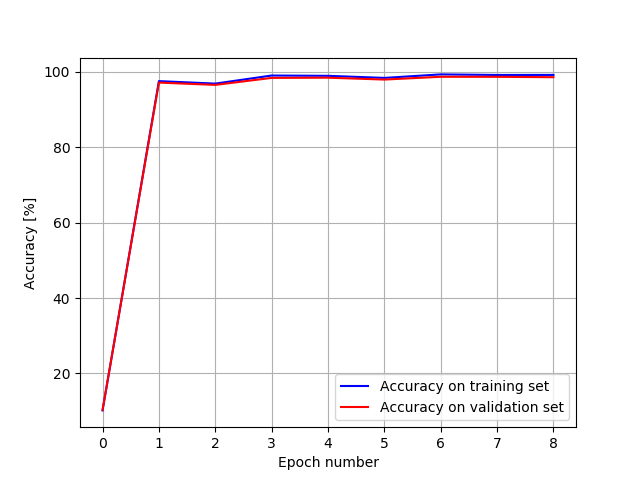
\includegraphics[scale=0.8]{hw2_py/results/_14_01_43/lr_0_01_net_1_CE_/accuracy_epoch.png}
	\captionof{figure}{Classification accuracy as a function of the Epoch number}
	\label{fig_4}
\end{minipage}
\vskip 0.1in
\end{enumerate}

Answering the step 6 question:
The classification accuracy reported is the following:
\begin{enumerate}
\item Training set: 99.186\%
\item Test set: 98.58 \%
\end{enumerate}

\newpage
\subsubsection{\textbf{b.}}
\textbf{This subsection answers the step 7 - part 1. }
\newline
First, we repeat the process with the different learning rate values, whereas all the other parameters defined in the previous subsection remain the same. And the results we get are the following:

\begin{enumerate}
\item For the same network with the learning rate of \textbf{0.1}:
\begin{enumerate}
\item Loss value graphs:

\vskip 0.1in
\begin{minipage}{\linewidth}
	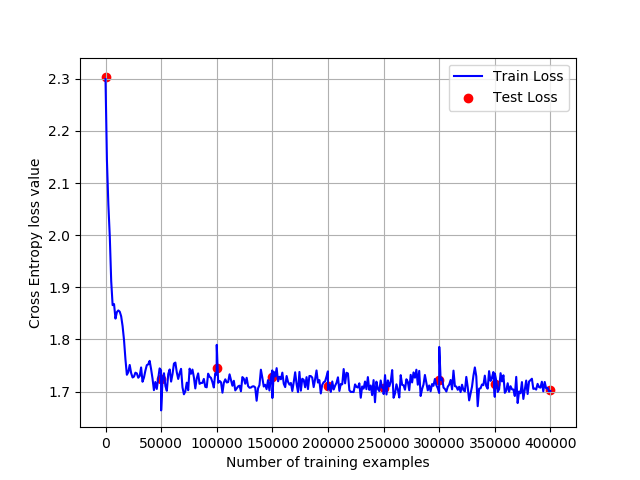
\includegraphics[scale=0.8]{hw2_py/results/_14_01_43/lr_0_1_net_1_CE_/loss_value.png}
	\captionof{figure}{Loss vs. Training examples}
	\label{fig_5}
\end{minipage}
\vskip 0.1in
\begin{minipage}{\linewidth}
	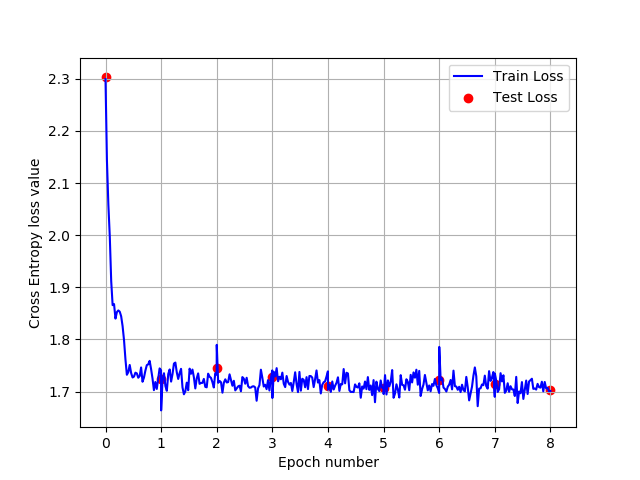
\includegraphics[scale=0.8]{hw2_py/results/_14_01_43/lr_0_1_net_1_CE_/loss_value_epoch.png}
	\captionof{figure}{Loss vs. Epoch number}
	\label{fig_6}
\end{minipage}
\vskip 0.1in

\item Classification accuracy graphs

\vskip 0.1in
\begin{minipage}{\linewidth}
	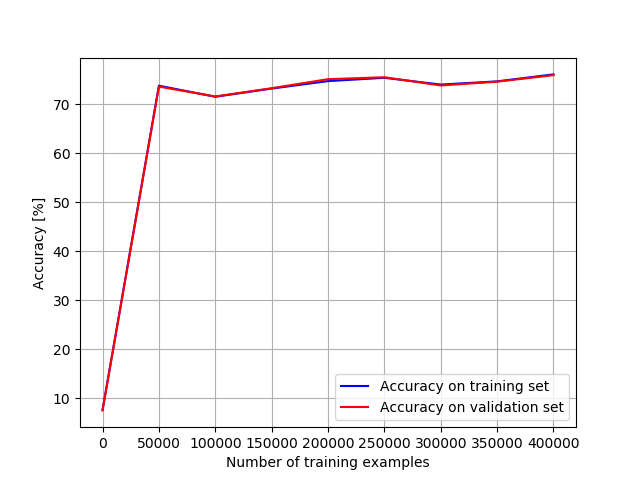
\includegraphics[scale=0.8]{hw2_py/results/_14_01_43/lr_0_1_net_1_CE_/accuracy.png}
	\captionof{figure}{ Accuracy vs. Training examples}
	\label{fig_7}
\end{minipage}
\vskip 0.1in
\begin{minipage}{\linewidth}
	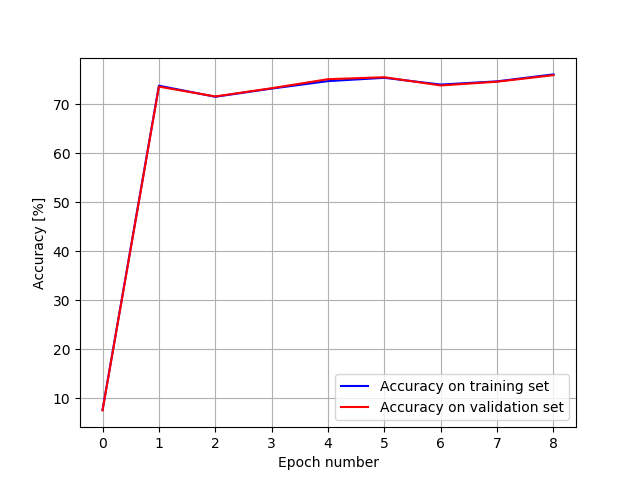
\includegraphics[scale=0.8]{hw2_py/results/_14_01_43/lr_0_1_net_1_CE_/accuracy_epoch.png}
	\captionof{figure}{Accuracy vs. Epoch number}
	\label{fig_8}
\end{minipage}
\vskip 0.1in






\end{enumerate}

\item For the same network with the learning rate of \textbf{0.0001}:


\begin{enumerate}

\item Loss value graphs:

\vskip 0.1in
\begin{minipage}{\linewidth}
	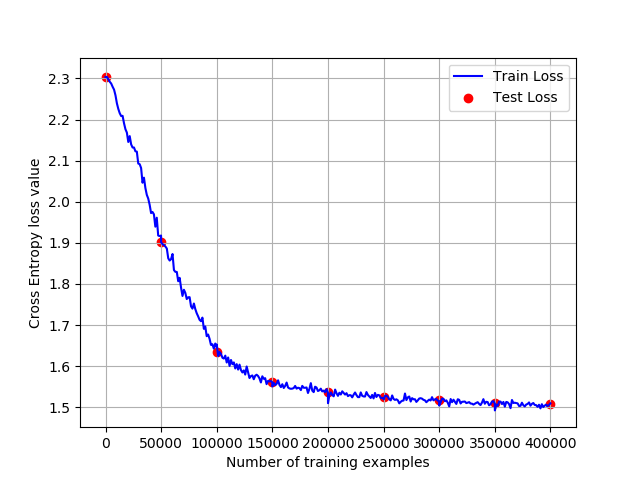
\includegraphics[scale=0.8]{hw2_py/results/_14_01_43/lr_0_0001_net_1_CE_/loss_value.png}
	\captionof{figure}{Loss vs. Training examples}
	\label{fig_9}
\end{minipage}
\vskip 0.1in
\begin{minipage}{\linewidth}
	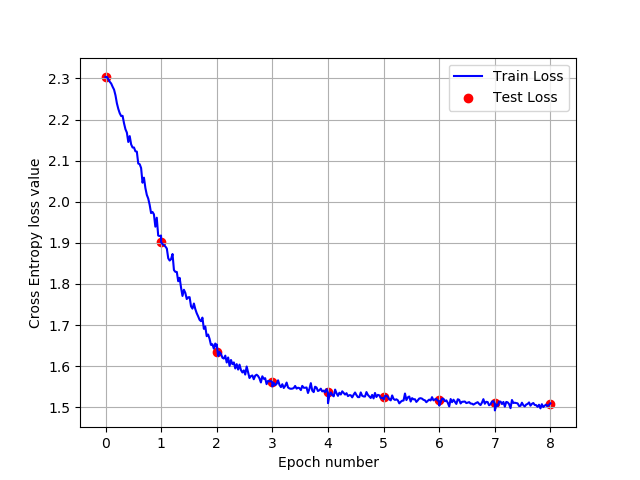
\includegraphics[scale=0.8]{hw2_py/results/_14_01_43/lr_0_0001_net_1_CE_/loss_value_epoch.png}
	\captionof{figure}{Loss vs. Epoch number}
	\label{fig_10}
\end{minipage}
\vskip 0.1in

\item Classification accuracy graphs

\vskip 0.1in
\begin{minipage}{\linewidth}
	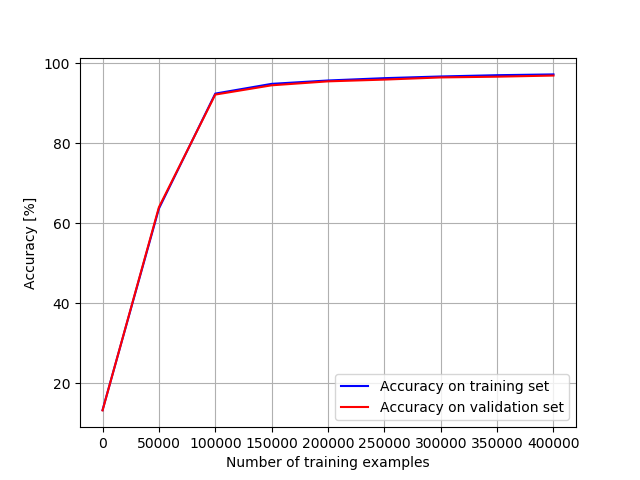
\includegraphics[scale=0.8]{hw2_py/results/_14_01_43/lr_0_0001_net_1_CE_/accuracy.png}
	\captionof{figure}{ Accuracy vs. Training examples}
	\label{fig_11}
\end{minipage}
\vskip 0.1in
\begin{minipage}{\linewidth}
	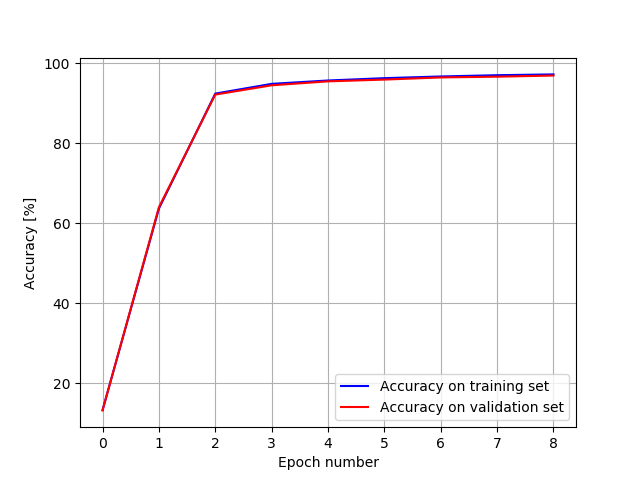
\includegraphics[scale=0.8]{hw2_py/results/_14_01_43/lr_0_0001_net_1_CE_/accuracy_epoch.png}
	\captionof{figure}{Accuracy vs. Epoch number}
	\label{fig_12}
\end{minipage}
\vskip 0.1in


\end{enumerate}

\end{enumerate}

\newpage
Answering the question asked, we compare the results and then draw conclusions. First, We compare the final accuracy on the validation set for 3 of the networks:

\begin{table}[]
\begin{tabular}{|l|l|l|}
\hline
Network LR & Final test accuracy {[}\%{]} & Final training accuracy {[}\%{]} \\ \hline
0.01       & 98.58                        & 99.186                           \\ \hline
0.1        & 75.88                        & 76.036                           \\ \hline
0.0001     & 96.94                        & 97.23                            \\ \hline
\end{tabular}
\end{table}


Then, we compare the accuracy of those 3 networks vs. the learning rate:

\vskip 0.1in
\begin{minipage}{\linewidth}
	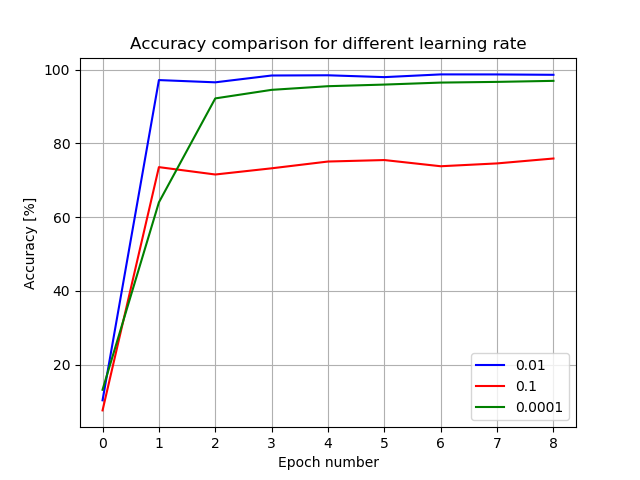
\includegraphics[scale=0.8]{{hw2_py/results/_14_01_43/comparison/accuracy_LR_1_2_3.png}}
	\captionof{figure}{Accuracy vs. Epoch number}
	\label{fig_13}
\end{minipage}
\vskip 0.1in


Several conclusions can be drawn from the overall results:

\begin{enumerate}
\item As we can see, the learning can is a parameter which has to be tuned in order to obtain optimal results:
\begin{enumerate}
\item Small learning rate leads to a network which will take a lot of time to converge, and this convergence will slow down even more when the Loss will decrease. We can see it in the case with $\alpha=0.0001$
\item Large learning rate may give a quick jump towards the optimal solution in the beginning, but the network may never converge, since the parameters will be changed very drastically, and the Loss will not decrease. We can see it in the case with $\alpha=0.1$ (which is high learning rate)
\end{enumerate}
There have been made a lot of research on this matter, and often the adaptive learning rate is being used. (which changes its value over time). From our example, over the given training time, the case with $\alpha = 0.01$ showed the best results
\item As mentioned above, the small learning rate makes small changes to the network parameter, so that the Loss value changes in a smooth way (Figure \ref{fig_10}). Opposite is true for the high learning rate (Figure \ref{fig_6})
\item As mentioned above, high learning rate will reach a point where is can no longer decrease the Loss value, since the changes made for the parameters are very big. This is visible good in the Figure \ref{fig_6}.
\item In all the cases, we can observe that the accuracy on the validation set is slightly smaller than the one on the training set. Which is logical, the network copes better with the data it has already seen and was trained on.

\end{enumerate}






\newpage
\subsubsection{\textbf{c.}}
\textbf{This subsection answers the step 7 - part 2. }
\newline
First, we repeat the process with the the same learning rate ($\alpha = 0.01$), but with a different Loss Function, using the L2 Norm function as the loss value. Reporting the same results, we obtain the following Loss valueand the following Accuracy graphs:

\begin{enumerate}

\item Loss value graphs:

\vskip 0.1in
\begin{minipage}{\linewidth}
	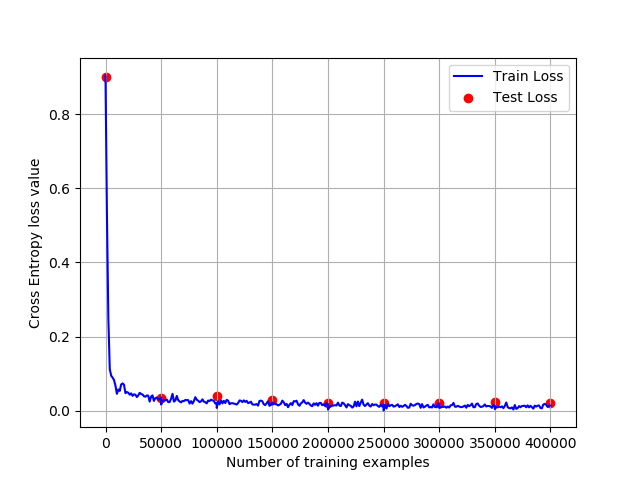
\includegraphics[scale=0.8]{hw2_py/results/_14_01_43/lr_0_01_net_1_L2_norm_/loss_value.png}
	\captionof{figure}{Loss vs. Training examples}
	\label{fig_14}
\end{minipage}
\vskip 0.1in
\begin{minipage}{\linewidth}
	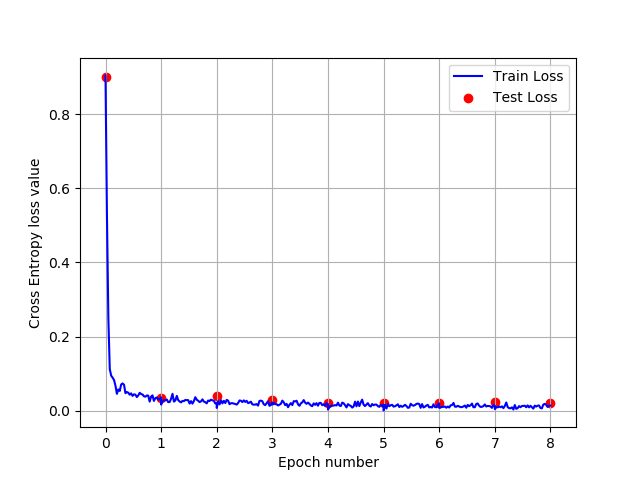
\includegraphics[scale=0.8]{hw2_py/results/_14_01_43/lr_0_01_net_1_L2_norm_/loss_value_epoch.png}
	\captionof{figure}{Loss vs. Epoch number}
	\label{fig_15}
\end{minipage}
\vskip 0.1in

\item Classification accuracy graphs

\vskip 0.1in
\begin{minipage}{\linewidth}
	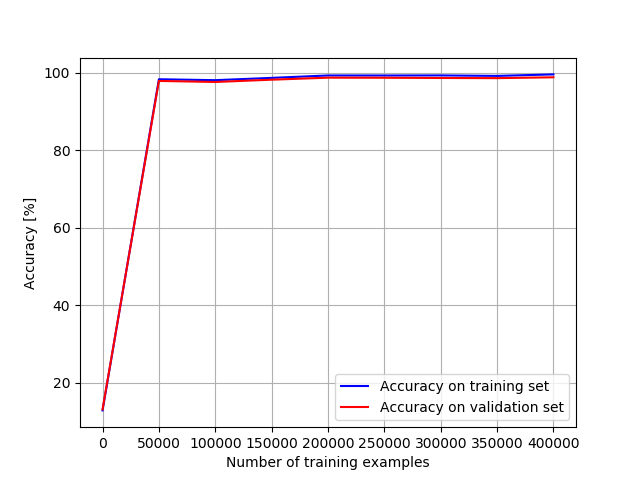
\includegraphics[scale=0.8]{hw2_py/results/_14_01_43/lr_0_01_net_1_L2_norm_/accuracy.png}
	\captionof{figure}{ Accuracy vs. Training examples}
	\label{fig_16}
\end{minipage}
\vskip 0.1in
\begin{minipage}{\linewidth}
	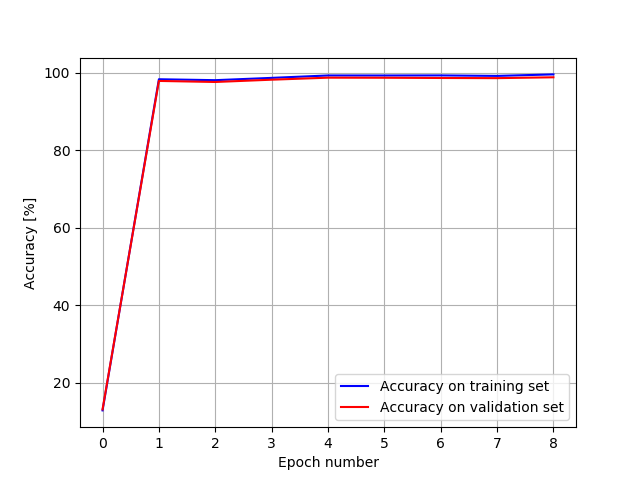
\includegraphics[scale=0.8]{hw2_py/results/_14_01_43/lr_0_01_net_1_L2_norm_/accuracy_epoch.png}
	\captionof{figure}{Accuracy vs. Epoch number}
	\label{fig_17}
\end{minipage}
\vskip 0.1in



\end{enumerate}

Comparing the accuracy rate on the trained network for both cases gives:

\begin{table}[]
\begin{tabular}{|l|l|l|}
\hline
Network Loss function & Final test accuracy {[}\%{]} & Final training accuracy {[}\%{]} \\ \hline
Cross Entropy         & 98.58                        & 99.186                           \\ \hline
N2 norm               & 98.77                        & 99.514                           \\ \hline
\end{tabular}
\end{table}


Then, we compare the accuracy of those 2 networks:
\vskip 0.1in
\begin{minipage}{\linewidth}
	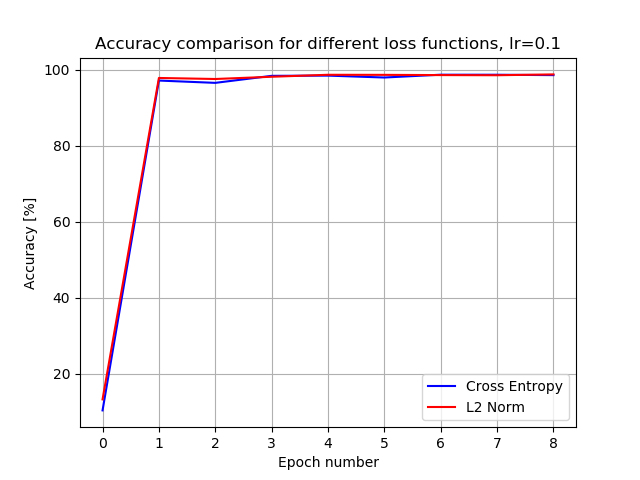
\includegraphics[scale=0.8]{hw2_py/results/_14_01_43/comparison/accuracy_1_4.png}
	\captionof{figure}{Accuracy vs. Epoch number}
	\label{fig_18}
\end{minipage}
\vskip 0.1in



Several conclusions can be drawn from the overall results:

\begin{enumerate}
\item As we can observe, there is no much difference in the performance of both networks, and both classify the validation examples approximately on the same level. Although this is the case in our example, choosing the correct Loss Function is vital for a successful Network training in other, more complex environments.
\end{enumerate}


\newpage
\subsubsection{\textbf{d.}}
\textbf{This subsection answers the step 8. }
\newline
First, we repeat the process with all the same parameters, but the network structure is different. The following results are being obtained (for the new network):

\begin{enumerate}
\item Loss value graphs:

\vskip 0.1in
\begin{minipage}{\linewidth}
	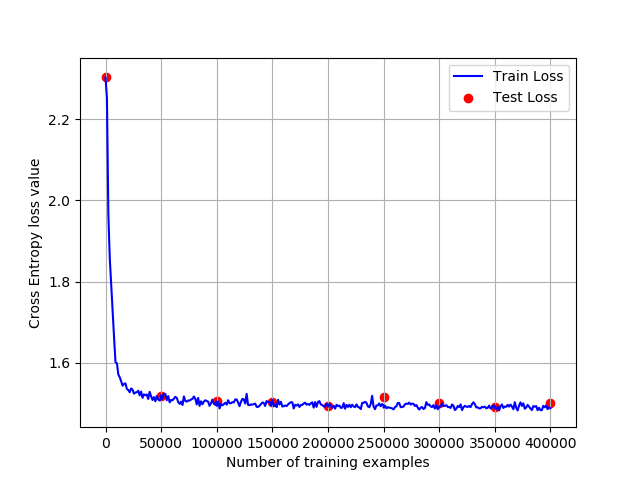
\includegraphics[scale=0.8]{hw2_py/results/_14_11_31/lr_0_01_net_2_CE_/loss_value.png}
	\captionof{figure}{Loss vs. Training examples}
	\label{fig_19}
\end{minipage}
\vskip 0.1in
\begin{minipage}{\linewidth}
	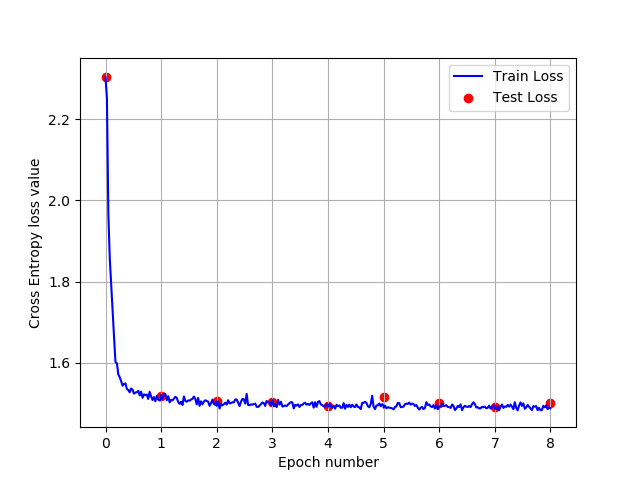
\includegraphics[scale=0.8]{hw2_py/results/_14_11_31/lr_0_01_net_2_CE_/loss_value_epoch.png}
	\captionof{figure}{Loss vs. Epoch number}
	\label{fig_20}
\end{minipage}
\vskip 0.1in

\item Classification accuracy graphs

\vskip 0.1in
\begin{minipage}{\linewidth}
	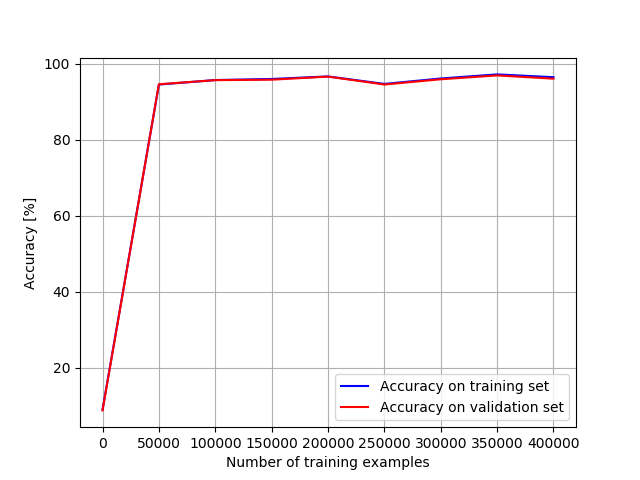
\includegraphics[scale=0.8]{hw2_py/results/_14_11_31/lr_0_01_net_2_CE_/accuracy.png}
	\captionof{figure}{ Accuracy vs. Training examples}
	\label{fig_21}
\end{minipage}
\vskip 0.1in
\begin{minipage}{\linewidth}
	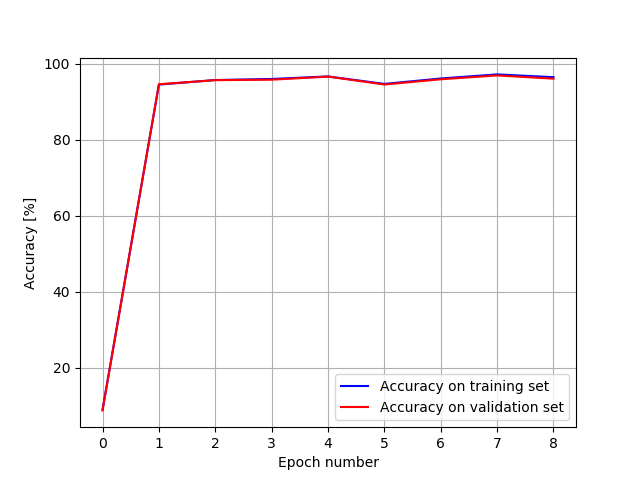
\includegraphics[scale=0.8]{hw2_py/results/_14_11_31/lr_0_01_net_2_CE_/accuracy_epoch.png}
	\captionof{figure}{Accuracy vs. Epoch number}
	\label{fig_22}
\end{minipage}
\vskip 0.1in

\end{enumerate}


Comparing the accuracy rate on the trained network for both cases gives:

\begin{table}[]
\begin{tabular}{|l|l|l|}
\hline
Network No. & Final test accuracy {[}\%{]} & Final training accuracy {[}\%{]} \\ \hline
1           & 98.76                        & 99.25                            \\ \hline
2           & 96.13                        & 96.52                            \\ \hline
\end{tabular}
\end{table}

\vskip 0.1in
\begin{minipage}{\linewidth}
	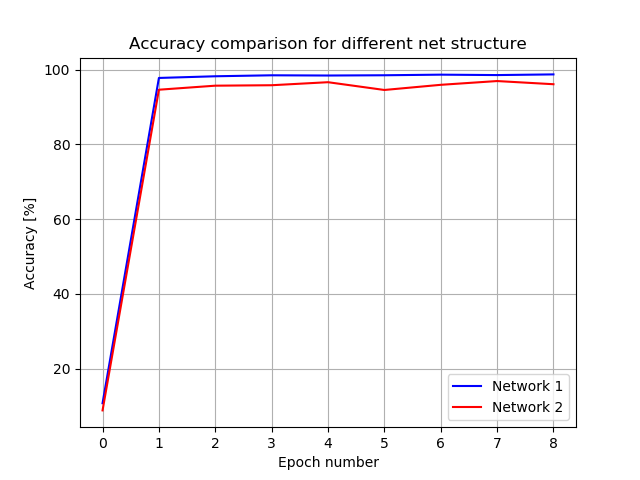
\includegraphics[scale=0.8]{hw2_py/results/_14_11_31/comparison/accuracy_1_5.png}
	\captionof{figure}{Accuracy vs. Epoch number}
	\label{fig_18}
\end{minipage}
\vskip 0.1in
Several conclusions can be drawn from the overall results:

\begin{enumerate}
\item As we can observe, the new network structure contains \textbf{less} parameters, which means, its performance abilities are smaller than from the network with more parameters. This is also one of the big considerations when creating the network architecture - finding the optimal amount of layers \& parameters / convolution size / etc. in each layer. From one side, the network should have enough parameters to supply the desired accuracy, from another side, an abundance of the parameters will lead to longer training time, and some other known problems (vanishing/exploding gradient, etc. ) 
\end{enumerate}



\newpage
\subsection{Question 2.}
\subsubsection{}
We have used the MATLAB version of the network, out of its simplicity to comply with the required tasks in this question. To run the code for this question, please run the \textbf{main.m} file inside the "matlab\_code" folder. 

\subsubsection{}
The bird images were loaded. Since their size differed from the input size to the VGG16 network ([224X224X3]), we had to resize them in order to fit into the network. This was done thoughtout the exercise without saving the Aspect Ratio of the images. The predictions for the birds are the following:

\vskip 0.1in
\begin{figure}
  \begin{subfigure}{0.4\linewidth}
	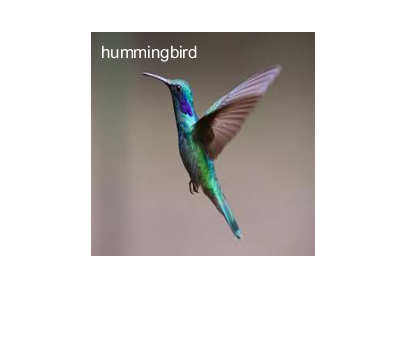
\includegraphics[width=\linewidth]{imgs/bird_0_labeled.png}
	\caption{Bird \#0 prediction}
  \end{subfigure}
  \begin{subfigure}{0.4\linewidth}
	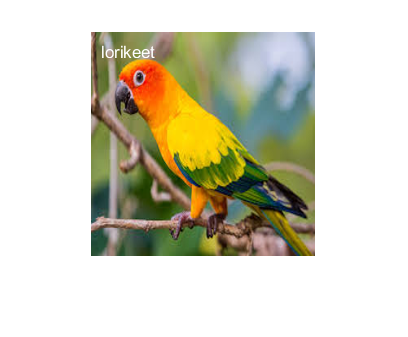
\includegraphics[width=\linewidth]{imgs/bird_1_labeled.png}
	\caption{Bird \#1 prediction}
  \end{subfigure}
\caption{Prediction on the input birds}
\end{figure}
\vskip 0.1in

As we can observe, the predictions are correct.


\subsubsection{}
The random image on the web that we have found is the image of the bear. The image was resized as well and has produced the following classification output, which is correct. (it says "Brown bear") (See Figure  \ref{Bear prediction} )

\vskip 0.1in
\begin{figure}[h!]
  \begin{subfigure}{0.4\linewidth}
	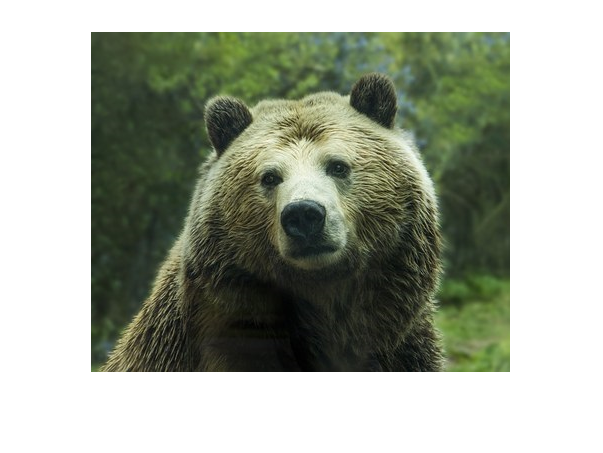
\includegraphics[width=\linewidth]{imgs/bear.png}
	\caption{Bear input image}
  \end{subfigure}
  \begin{subfigure}{0.4\linewidth}
	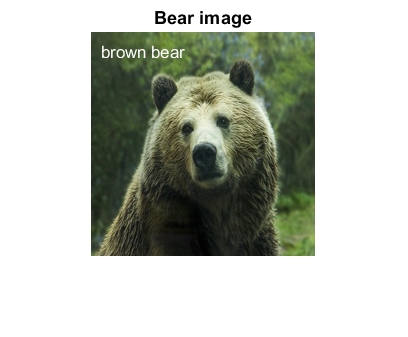
\includegraphics[width=\linewidth]{imgs/bear_classified.png}
	\caption{Bear resized and classified}
  \end{subfigure}
\caption{Bear prediction}
\label{Bear prediction}
\end{figure}
\vskip 0.1in

\subsubsection{}
The following transformations have been applied:

\begin{enumerate}
\item \textbf{Geometric transformation: } we have used the 'shear', which is represented by the following affine transformation matrix:

\begin{equation*}
\text{shear matrix used: }
\left[
\begin{matrix}
1 & 0 & 0 \\
0.45 & 1 & 0 \\
0 & 0 & 1
\end{matrix}
\right]
\end{equation*}

\item \textbf{Color transformation: } we have affected the Hue channel, multiplying its values by 2.5
\item \textbf{Filter: } we used the Motion Blur filter defined in MATLAB, of size 20, with angle of 45 degrees
\end{enumerate}

The results are presented in the next image. As we can see, all the classifications are still correct, which signals that the network is robust enough to all those modifications. (See Figure  \ref{Bear modified predictions} )  We can also observe, than in comparison to not modified bear image, the prediction certaintly was slightly decreased, where the most reduction was for the blurred image of the bear


\vskip 0.1in
\begin{figure}
  \begin{subfigure}{0.4\linewidth}
	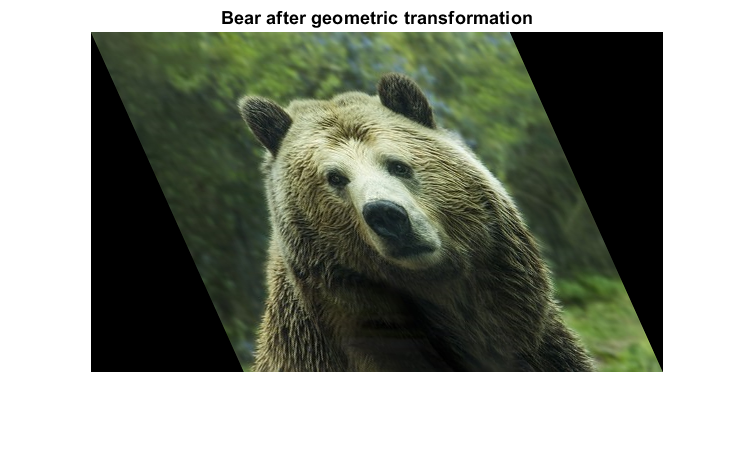
\includegraphics[width=\linewidth]{imgs/bear_sheared.png}
	\caption{Bear sheared input image}
  \end{subfigure}
  \begin{subfigure}{0.4\linewidth}
	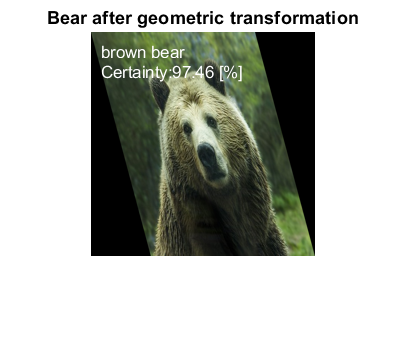
\includegraphics[width=\linewidth]{imgs/bear_sheared_classified.png}
	\caption{Bear sheared classified}
  \end{subfigure}

  \begin{subfigure}{0.4\linewidth}
	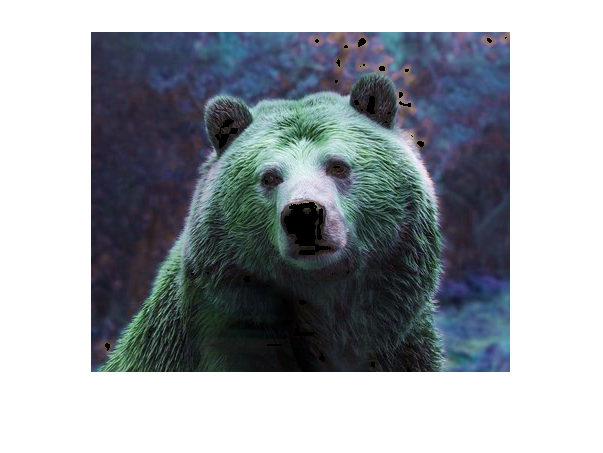
\includegraphics[width=\linewidth]{imgs/bear_hue.png}
	\caption{Modified color bear}
  \end{subfigure}
  \begin{subfigure}{0.4\linewidth}
	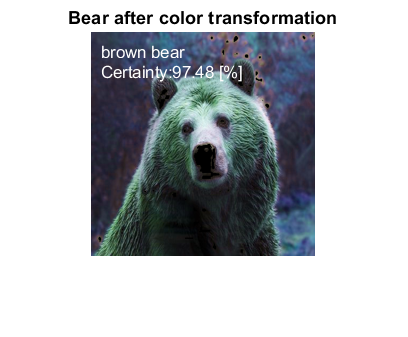
\includegraphics[width=\linewidth]{imgs/bear_hue_classified.png}
	\caption{Modified color bear classified}
  \end{subfigure}

  \begin{subfigure}{0.4\linewidth}
	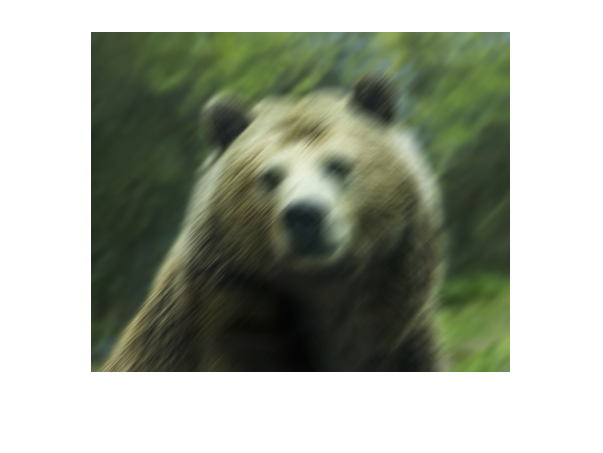
\includegraphics[width=\linewidth]{imgs/bear_blurred.png}
	\caption{Blurred bear}
  \end{subfigure}
  \begin{subfigure}{0.4\linewidth}
	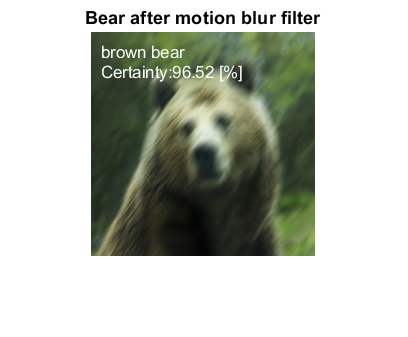
\includegraphics[width=\linewidth]{imgs/bear_blurred_classified.png}
	\caption{Blurred bear classified}
  \end{subfigure}


\caption{Bear modifications and its prediction}
\label{Bear modified predictions}
\end{figure}
\vskip 0.1in






\subsubsection{}
The filters in the first convolution layer are of the size [3X3X3], which means that the single filter on the input image [224X224X3] produces 1 output image [224X224X1], which is easy to vizualize.
\newline
The filters chosen randomly are 5 and 32. To vizualize the filters, their values were normalized (to fit into [0 1] range), and then viewed. The 3 depth layers are being presented as 3 2D filters. (but each filter is [3X3X3]). Filters are presented in Figure \ref{Filters}:

\vskip 0.1in
\begin{figure}[!htbp]
	\begin{subfigure}{0.6\linewidth}
		\centering
		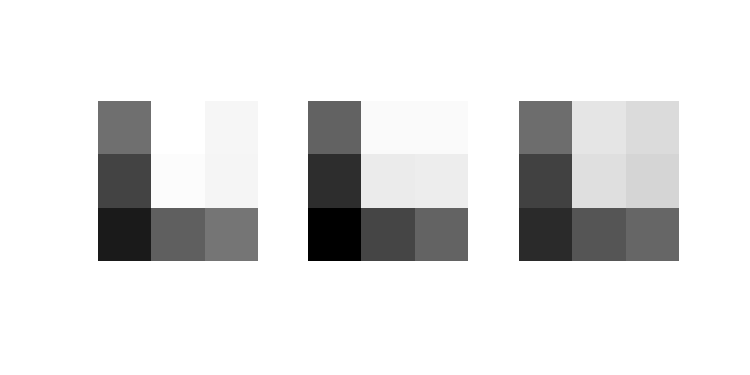
\includegraphics[width=\linewidth]{imgs/filter_1.png}
		\caption{Filter 1}
	\end{subfigure}
	\vskip 0.1in
	\begin{subfigure}{0.6\linewidth}
		\centering
		
\includegraphics[width=\linewidth]{imgs/filter_2.png}
		\caption{Filter 2}
	\end{subfigure}
	\caption{Filters 5 and 32}
	\label{Filters}
\end{figure}
\vskip 0.1in

As we can observe, Filter 1 is trained to detect edges. Filter 2 detects places which have more light, where the texture is more visible.

The responses of each of the input images are presented in the Figure \ref{Filters_responses}, where the left column provides the responses for Filter 1, and the right - for Filter 2. So we can see the differences more clearly, the responses to the original bear image are also presented there


\vskip 0.1in
\begin{figure}

  \begin{subfigure}{0.4\linewidth}
	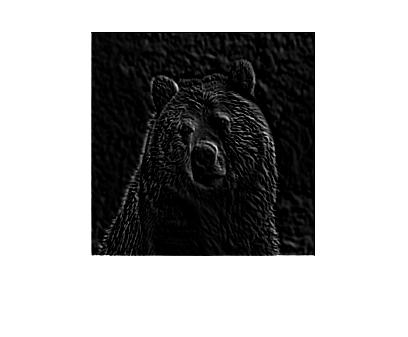
\includegraphics[width=\linewidth]{imgs/response_filt_1.png}
	\caption{Bear original response to Filter 1}
  \end{subfigure}
  \begin{subfigure}{0.4\linewidth}
	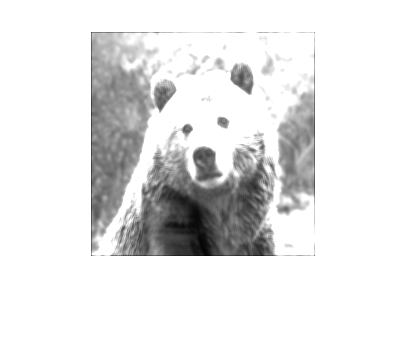
\includegraphics[width=\linewidth]{imgs/response_filt_2.png}
	\caption{Bear original response to Filter 2}
  \end{subfigure}


  \begin{subfigure}{0.4\linewidth}
	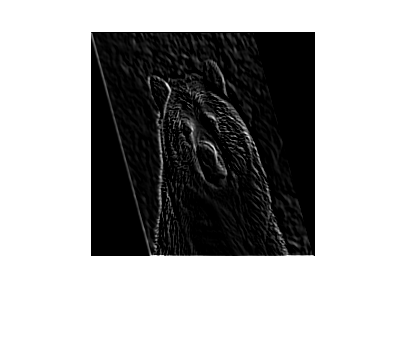
\includegraphics[width=\linewidth]{imgs/bear_sheared_filtered_1.png}
	\caption{Bear sheared response to Filter 1}
  \end{subfigure}
  \begin{subfigure}{0.4\linewidth}
	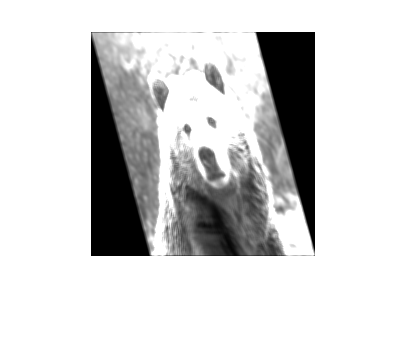
\includegraphics[width=\linewidth]{imgs/bear_sheared_filtered_2.png}
	\caption{Bear sheared response to Filter 2}
  \end{subfigure}

  \begin{subfigure}{0.4\linewidth}
	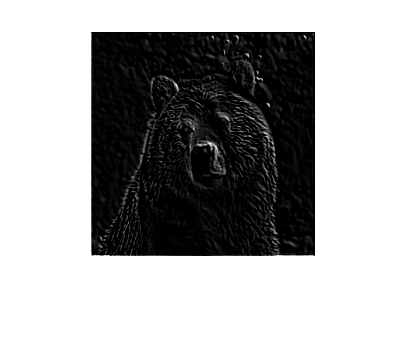
\includegraphics[width=\linewidth]{imgs/bear_hued_filtered_1.png}
	\caption{Bear hue transformed response to Filter 1}
  \end{subfigure}
  \begin{subfigure}{0.4\linewidth}
	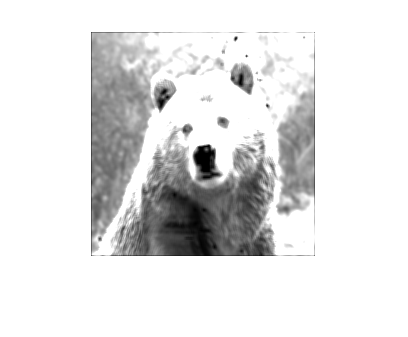
\includegraphics[width=\linewidth]{imgs/bear_hued_filtered_2.png}
	\caption{Bear hue transformed response to Filter 2}
  \end{subfigure}

  \begin{subfigure}{0.4\linewidth}
	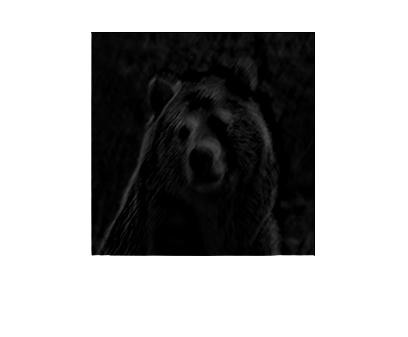
\includegraphics[width=\linewidth]{imgs/bear_blurred_filtered_1.png}
	\caption{Bear blurred response to Filter 1}
  \end{subfigure}
  \begin{subfigure}{0.4\linewidth}
	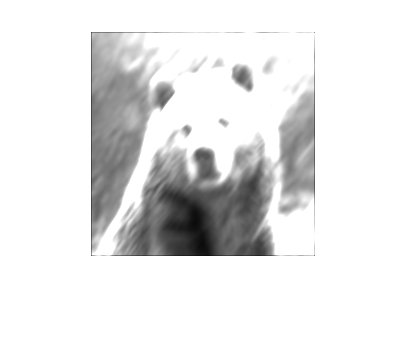
\includegraphics[width=\linewidth]{imgs/bear_blurred_filtered_2.png}
	\caption{Bear blurred response to Filter 2}
  \end{subfigure}


\caption{Transformed bear image responses to filters}
\label{Filters_responses}
\end{figure}
\vskip 0.1in



Some information on the image responses to the first layers in the CNN:
"These images mostly contain edges and colors, which indicates that the filters at layer 'conv1' are edge detectors and color filters. The edge detectors are at different angles, which allows the network to construct more complex features in the later layers."\footnote{https://www.mathworks.com/help/deeplearning/examples/visualize-features-of-a-convolutional-neural-network.html }

By looking at the differences we can say the following:

\begin{enumerate}
\item We can see that the Filter 1 is the edge detector, while the Filter 2 also responses to the Color.
\item Blurring of the image makes it harder to detect edges, and they become mich more vague
\item The Hue change affects the second filter output a bit
\item The shear has affected the Filter 1 response - the edges detected are now at different angle. Some are detected more, some are less
\end{enumerate}



\subsubsection{}
Every image of cats and dogs was passed through the network, the Feature vectors of size 4096 were obtained for each image. Using the PCA method, the Principal Components were obtained and the Principal Component Scores for each of the samples (dogs, cats). The graphs below show the clusters of cats and dogs. It may be seen that there is a certain difference between the two. It was observed that the 3rd PC also was large, in relation to PC1 and PC2. Thus, a 3D scatter plot is also presented: (Figure \ref{PC_graphs})

\vskip 0.1in
\begin{figure}[!htbp]
	\begin{subfigure}{0.8\linewidth}
		\centering
		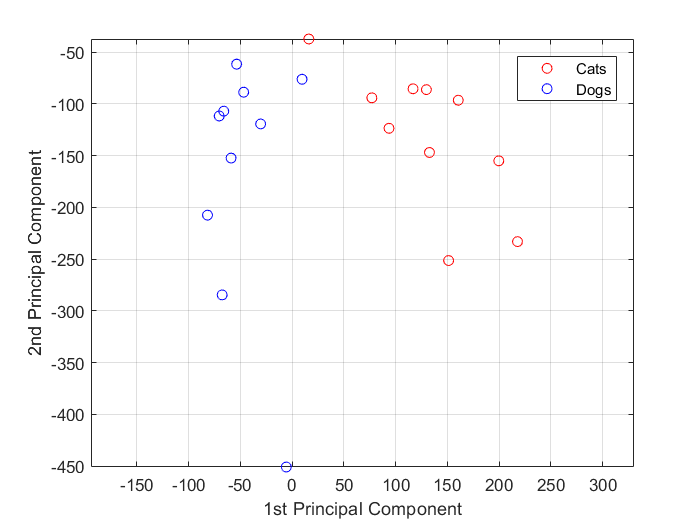
\includegraphics[width=\linewidth]{imgs/scatter_2d_pca.png}
		\caption{PCA with 2 PC}
	\end{subfigure}
	\vskip 0.1in
	\begin{subfigure}{0.8\linewidth}
		\centering
		\includegraphics[width=\linewidth]{imgs/scatter_3d_pca.png}
		\caption{PCA with 3 PC}
	\end{subfigure}
	\caption{PCA Scores graphs for cats and dogs}
	\label{PC_graphs}
\end{figure}
\vskip 0.1in


\subsubsection{}
The images of a cat and a dog from the internet are preseted in the Figure \ref{a Cat and a Dog new images}. The coefficienct of the PCA transformation from previous question were used to obtain the PC scores for the new images. The new images are being displayed on the same PC scores graph (both 2D and 3D) and are presented in Figure \ref{new Cat and Dog images in PC scores graphs}. Then, the closest neighbor was found for both a cat and a dog through the Minimal Euclidean Distance (L2) (over the vector of all 20 features).  The closest image of a cat with a new cat and the closest image of a dog are presented in \ref{closest_cat_dog_images}. We can indeed notice that the pairs match and look similar.

\vskip 0.1in
\begin{figure}[!htbp]
	\begin{subfigure}{0.4\linewidth}
		\centering
		\includegraphics[width=\linewidth,scale=0.8]{imgs/cat.jpg}
		\caption{a new cat image}
	\end{subfigure}
	\begin{subfigure}{0.4\linewidth}
		\centering
		\includegraphics[width=\linewidth,scale=0.8]{imgs/dog.jpg}
		\caption{a new dog image}
	\end{subfigure}
	\caption{a Cat and a Dog new images}
	\label{a Cat and a Dog new images}
\end{figure}
\vskip 0.1in

\vskip 0.1in
\begin{figure}[!htbp]
	\begin{subfigure}{0.8\linewidth}
		\centering
		\includegraphics[width=\linewidth]{imgs/scatter_2d_new_imgs.png}
		\caption{PCA with 2 PC}
	\end{subfigure}
	\vskip 0.1in
	\begin{subfigure}{0.8\linewidth}
		\centering
		\includegraphics[width=\linewidth]{imgs/scatter_3d_new_imgs.png}
		\caption{PCA with 3 PC}
	\end{subfigure}
	\caption{new Cat and Dog images in PC scores graphs}
	\label{new Cat and Dog images in PC scores graphs}
\end{figure}
\vskip 0.1in


\vskip 0.1in
\begin{figure}[!htbp]
	\begin{subfigure}{0.4\linewidth}
		\centering
		\includegraphics[width=\linewidth,scale=0.8]{imgs/cat.jpg}
		\caption{a new cat image}
	\end{subfigure}
	\begin{subfigure}{0.4\linewidth}
		\centering
		\includegraphics[width=\linewidth,scale=0.8]{imgs/cat_8.jpg}
		\caption{cat from library - cat\_8}
	\end{subfigure}

	\begin{subfigure}{0.4\linewidth}
		\centering
		\includegraphics[width=\linewidth,scale=0.8]{imgs/dog.jpg}
		\caption{a new dog image}
	\end{subfigure}
	\begin{subfigure}{0.4\linewidth}
		\centering
		\includegraphics[width=\linewidth,scale=0.8]{imgs/dog_5.jpg}
		\caption{dog from library - dog\_5)}
	\end{subfigure}


	\caption{Closest cats and dogs images}
	\label{closest_cat_dog_images}
\end{figure}
\vskip 0.1in




\subsubsection{}
The same procedure is being done for the random tiger and wolf images from the internet. You can see the results in the figures:

\begin{enumerate}
\item PCA score graphs with new tiger and wolf images: Figure \ref{PCA_tiger_wolf}
\item The closest image to the tiger and to the wolf: Figure \ref{Closest_tiger_wolf} 
\end{enumerate}
We can see from the PC scores graph that the tiger and the wolf sit a bit further away from the cats and dogs clusters. The images of the closest cats and dogs do resemble the wolf and the tiger (the most, from all the other cats and dogs images). The cat has the similar texture, and the dog...has similar pose, face shape, ears, and the face texture.



\vskip 0.1in
\begin{figure}[!htbp]
	\begin{subfigure}{0.8\linewidth}
		\centering
		\includegraphics[width=\linewidth]{imgs/scatter_2d_tiger_wolf.png}
		\caption{PCA with 2 PC}
	\end{subfigure}
	\vskip 0.1in
	\begin{subfigure}{0.8\linewidth}
		\centering
		\includegraphics[width=\linewidth]{imgs/scatter_3d_tiger_wolf.png}
		\caption{PCA with 3 PC}
	\end{subfigure}
	\caption{Tiger and Wolf PCA scores on existing PCA graph}
	\label{PCA_tiger_wolf}
\end{figure}
\vskip 0.1in


\vskip 0.1in
\begin{figure}[!htbp]
	\begin{subfigure}{0.4\linewidth}
		\centering
		\includegraphics[width=\linewidth,scale=0.8]{imgs/tiger.jpg}
		\caption{Tiger}
	\end{subfigure}
	\begin{subfigure}{0.4\linewidth}
		\centering
		\includegraphics[width=\linewidth,scale=0.8]{imgs/cat_7.jpg}
		\caption{cat from library - cat\_7}
	\end{subfigure}

	\begin{subfigure}{0.4\linewidth}
		\centering
		\includegraphics[width=\linewidth,scale=0.8]{imgs/wolf.jpg}
		\caption{Wolf}
	\end{subfigure}
	\begin{subfigure}{0.4\linewidth}
		\centering
		\includegraphics[width=\linewidth,scale=0.8]{imgs/dog_7.jpg}
		\caption{dog from library - dog\_7}
	\end{subfigure}


	\caption{Closest cats and dogs images}
	\label{Closest_tiger_wolf} 
\end{figure}
\vskip 0.1in




\AtEndDocument{\section{Image Stitching}\includepdf[pages=-]{cv_hw2.pdf}}



\end{document}



















